% Created by tikzDevice version 0.12.3.1 on 2021-12-06 11:02:55
% !TEX encoding = UTF-8 Unicode
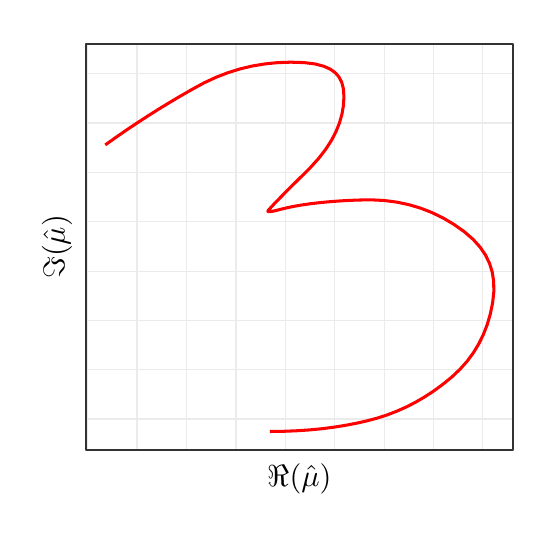
\begin{tikzpicture}[x=1pt,y=1pt]
\definecolor{fillColor}{RGB}{255,255,255}
\begin{scope}
\definecolor{drawColor}{RGB}{255,255,255}
\definecolor{fillColor}{RGB}{255,255,255}

\path[draw=drawColor,line width= 0.6pt,line join=round,line cap=round,fill=fillColor] (  0.00,  3.84) rectangle (180.67,176.84);
\end{scope}
\begin{scope}
\definecolor{fillColor}{RGB}{255,255,255}

\path[fill=fillColor] ( 20.71, 24.55) rectangle (175.17,171.34);
\definecolor{drawColor}{gray}{0.92}

\path[draw=drawColor,line width= 0.3pt,line join=round] ( 20.71, 53.52) --
	(175.17, 53.52);

\path[draw=drawColor,line width= 0.3pt,line join=round] ( 20.71, 89.22) --
	(175.17, 89.22);

\path[draw=drawColor,line width= 0.3pt,line join=round] ( 20.71,124.91) --
	(175.17,124.91);

\path[draw=drawColor,line width= 0.3pt,line join=round] ( 20.71,160.60) --
	(175.17,160.60);

\path[draw=drawColor,line width= 0.3pt,line join=round] ( 21.37, 24.55) --
	( 21.37,171.34);

\path[draw=drawColor,line width= 0.3pt,line join=round] ( 57.07, 24.55) --
	( 57.07,171.34);

\path[draw=drawColor,line width= 0.3pt,line join=round] ( 92.76, 24.55) --
	( 92.76,171.34);

\path[draw=drawColor,line width= 0.3pt,line join=round] (128.45, 24.55) --
	(128.45,171.34);

\path[draw=drawColor,line width= 0.3pt,line join=round] (164.15, 24.55) --
	(164.15,171.34);

\path[draw=drawColor,line width= 0.6pt,line join=round] ( 20.71, 35.68) --
	(175.17, 35.68);

\path[draw=drawColor,line width= 0.6pt,line join=round] ( 20.71, 71.37) --
	(175.17, 71.37);

\path[draw=drawColor,line width= 0.6pt,line join=round] ( 20.71,107.06) --
	(175.17,107.06);

\path[draw=drawColor,line width= 0.6pt,line join=round] ( 20.71,142.76) --
	(175.17,142.76);

\path[draw=drawColor,line width= 0.6pt,line join=round] ( 39.22, 24.55) --
	( 39.22,171.34);

\path[draw=drawColor,line width= 0.6pt,line join=round] ( 74.91, 24.55) --
	( 74.91,171.34);

\path[draw=drawColor,line width= 0.6pt,line join=round] (110.61, 24.55) --
	(110.61,171.34);

\path[draw=drawColor,line width= 0.6pt,line join=round] (146.30, 24.55) --
	(146.30,171.34);
\definecolor{drawColor}{RGB}{255,0,0}

\path[draw=drawColor,line width= 1.1pt,line join=round] ( 87.20, 31.22) --
	( 92.14, 31.29) --
	( 96.91, 31.48) --
	(101.50, 31.79) --
	(105.94, 32.21) --
	(110.21, 32.76) --
	(114.34, 33.41) --
	(118.33, 34.17) --
	(122.17, 35.03) --
	(125.90, 36.02) --
	(129.53, 37.18) --
	(133.07, 38.54) --
	(136.53, 40.09) --
	(139.93, 41.83) --
	(143.27, 43.79) --
	(146.57, 45.95) --
	(149.82, 48.34) --
	(153.02, 50.96) --
	(155.93, 53.72) --
	(158.49, 56.60) --
	(160.73, 59.63) --
	(162.67, 62.82) --
	(164.34, 66.20) --
	(165.74, 69.80) --
	(166.87, 73.65) --
	(167.72, 77.79) --
	(168.15, 81.86) --
	(168.08, 85.53) --
	(167.55, 88.90) --
	(166.57, 92.03) --
	(165.12, 94.99) --
	(163.17, 97.85) --
	(160.64,100.66) --
	(157.44,103.43) --
	(153.64,106.10) --
	(149.74,108.41) --
	(145.75,110.34) --
	(141.66,111.93) --
	(137.43,113.19) --
	(133.03,114.11) --
	(128.44,114.70) --
	(123.61,114.94) --
	(118.56,114.84) --
	(113.79,114.61) --
	(109.44,114.31) --
	(105.49,113.94) --
	(101.91,113.53) --
	( 98.69,113.06) --
	( 95.81,112.56) --
	( 93.23,112.02) --
	( 90.95,111.46) --
	( 89.14,111.00) --
	( 87.91,110.75) --
	( 87.15,110.66) --
	( 86.74,110.66) --
	( 86.55,110.71) --
	( 86.50,110.78) --
	( 86.52,110.90) --
	( 86.66,111.14) --
	( 87.02,111.56) --
	( 87.60,112.20) --
	( 88.44,113.11) --
	( 89.60,114.32) --
	( 91.12,115.88) --
	( 93.05,117.83) --
	( 95.45,120.23) --
	( 98.36,123.11) --
	(101.77,126.49) --
	(104.85,129.90) --
	(107.41,133.21) --
	(109.48,136.43) --
	(111.12,139.59) --
	(112.37,142.72) --
	(113.25,145.84) --
	(113.79,148.98) --
	(113.98,152.19) --
	(113.78,155.09) --
	(113.18,157.40) --
	(112.23,159.26) --
	(110.91,160.81) --
	(109.13,162.10) --
	(106.76,163.18) --
	(103.64,164.01) --
	( 99.59,164.52) --
	( 94.73,164.67) --
	( 89.95,164.50) --
	( 85.32,164.03) --
	( 80.80,163.27) --
	( 76.38,162.22) --
	( 72.03,160.86) --
	( 67.75,159.21) --
	( 63.50,157.23) --
	( 59.28,154.94) --
	( 55.11,152.55) --
	( 51.01,150.12) --
	( 46.97,147.66) --
	( 43.00,145.15) --
	( 39.10,142.61) --
	( 35.25,140.04) --
	( 31.46,137.42) --
	( 27.74,134.77);
\definecolor{drawColor}{gray}{0.20}

\path[draw=drawColor,line width= 0.6pt,line join=round,line cap=round] ( 20.71, 24.55) rectangle (175.17,171.34);
\end{scope}
\begin{scope}
\definecolor{drawColor}{RGB}{0,0,0}

\node[text=drawColor,anchor=base,inner sep=0pt, outer sep=0pt, scale=  1.10] at ( 97.94, 11.47) {$\Re(\hat\mu)$};
\end{scope}
\begin{scope}
\definecolor{drawColor}{RGB}{0,0,0}

\node[text=drawColor,rotate= 90.00,anchor=base,inner sep=0pt, outer sep=0pt, scale=  1.10] at ( 13.08, 97.94) {$\Im(\hat\mu)$};
\end{scope}
\end{tikzpicture}
